% ************************************************************************
%
% Introduction
%
% ************************************************************************
\chpos{22mm}{10mm}

\chapter[Introduction]{Introduction}
\markboth{\thechapter\ \ Introduction}{\thechapter\ \ Introduction}
\label{ch1:introduction}

%\mysquote{0.8\textwidth}{Quote text.}{Author (\oldstylenums{1000} - \oldstylenums{1100})}

% ************************************************************************
%https://www.quantamagazine.org/why-the-first-drawings-of-neurons-were-defaced-20170928/
%https://www.npr.org/sections/health-shots/2017/01/26/511455876/art-exhibition-celebrates-drawings-by-the-founder-of-modern-neuroscience
%https://www.nytimes.com/2018/01/18/arts/design/brain-neuroscience-santiago-ramon-y-cajal-grey-gallery.html
%https://www.brainpickings.org/2017/02/23/beautiful-brain-santiago-ramon-y-cajal/
\section{Neuron cell reconstruction} % 
\lettrine{F}{ascination} with the neuron cells dates to the pioneering investigation over a century ago when a glance into the sample of silver-stained brain tissue made it possible to disclose the intricate network that forms the very essence of the nervous system. Remarkable milestone drawings of Santiago Ram\'{o}n y Cajal \cite{ramon2008histologia} - the founding father of neuroscience, remain as vivid as the images acquired by the latest state-of-the-art fluorescence microscope. Ever since the breakthrough, numerous studies \cite{ascoli2001computer,defelipe2002microstructure,defelipe1992pyramidal,van2001need,scorcioni2004quantitative,mason2007initiation,gensel2010semi,markram2015reconstruction} have practiced using morphological features of the neurons to gain a deeper insight into various aspects of the functionality. Today seen as revolutionary, hundred years old hand-made illustrations depicting microscope-magnified samples of the brain tissue \cite{swanson2017} displayed exceptional level of detail. The insights comparable to the ones provided with the modern expert-assisted digital reconstructions obtained using the latest equipment, rendered with the newest computer graphics. For the years that came the discipline gradually established as neuroscience \cite{kandel2000principles}. Furthermore, the astounding advancement of electrical engineering and computer science laid out the foundations for more specialized disciplines such as neuroinformatics and neural engineering (Fig.~\ref{ch1_fig1}). Recently, the attention is directed towards brain science - domain dedicated to the investigation of the captivating mechanism of, arguably, one of the most complex and mysterious organs. The disclosure of Cajal's groundbreaking \textit{neuron doctrine}\footnote{Every neuron in the brain is separate. Neuron cells conduct information in a defined direction and communicate across the synapses \cite{glickstein2006golgi}.} brought to light the idea that the nervous system is a network composed of the building blocks called neuron cells. Each cell (Fig.~\ref{ch1_fig7}) further represents sophisticated, interconnected processing component that both transmit and process the information. Different cells have different roles and hence varying properties, including the topology. The network structure is very important and offers the possibility to grasp useful evidences related to the functionality.

Physical materialization of the cell portrays the inner structure of the neuronal tissue and yields a valuable insight into the mechanisms behind the nervous system. Various studies have been carried out in order to understand neuron behavior and further unravel the underlying principles. Hence, the knowledge of neuron morphology provides with an essential resource for specialized analysis that can typically include (examination of the changes in neuronal structure) (reactions, studying response) caused by the external stimuli \cite{gomez2007immobilized,koppes2011neurite}, modeling \cite{ascoli2001computer}, statistical analysis \cite{polavaram2014statistical}, describing connectivity patterns \cite{}, cataloging neuron phenotypes (identities) \cite{defelipe2013new}, classification of neuron types \cite{armananzas2015towards}, simulating electrophysiological behavior \cite{} or the statistical analysis \cite{samsonovich2005statistical}. Widely used Sholl analysis methodology \cite{sholl1953dendritic} makes the direct use of the digital neuron reconstructions as a blue print of the morphology. It is commonly used in neuroscientific experimentation for quantitative analysis of the morphological characteristics of the neuron \cite{garcia2014new}. Aforenamed neuroscientific studies directly rely on accurate knowledge of 3D neuronal morphology which can not be depicted with a raw data image stack but requires comprehensive and precise specification \cite{parekh2013neuronal}.

\begin{figure}
	\begin{center}
		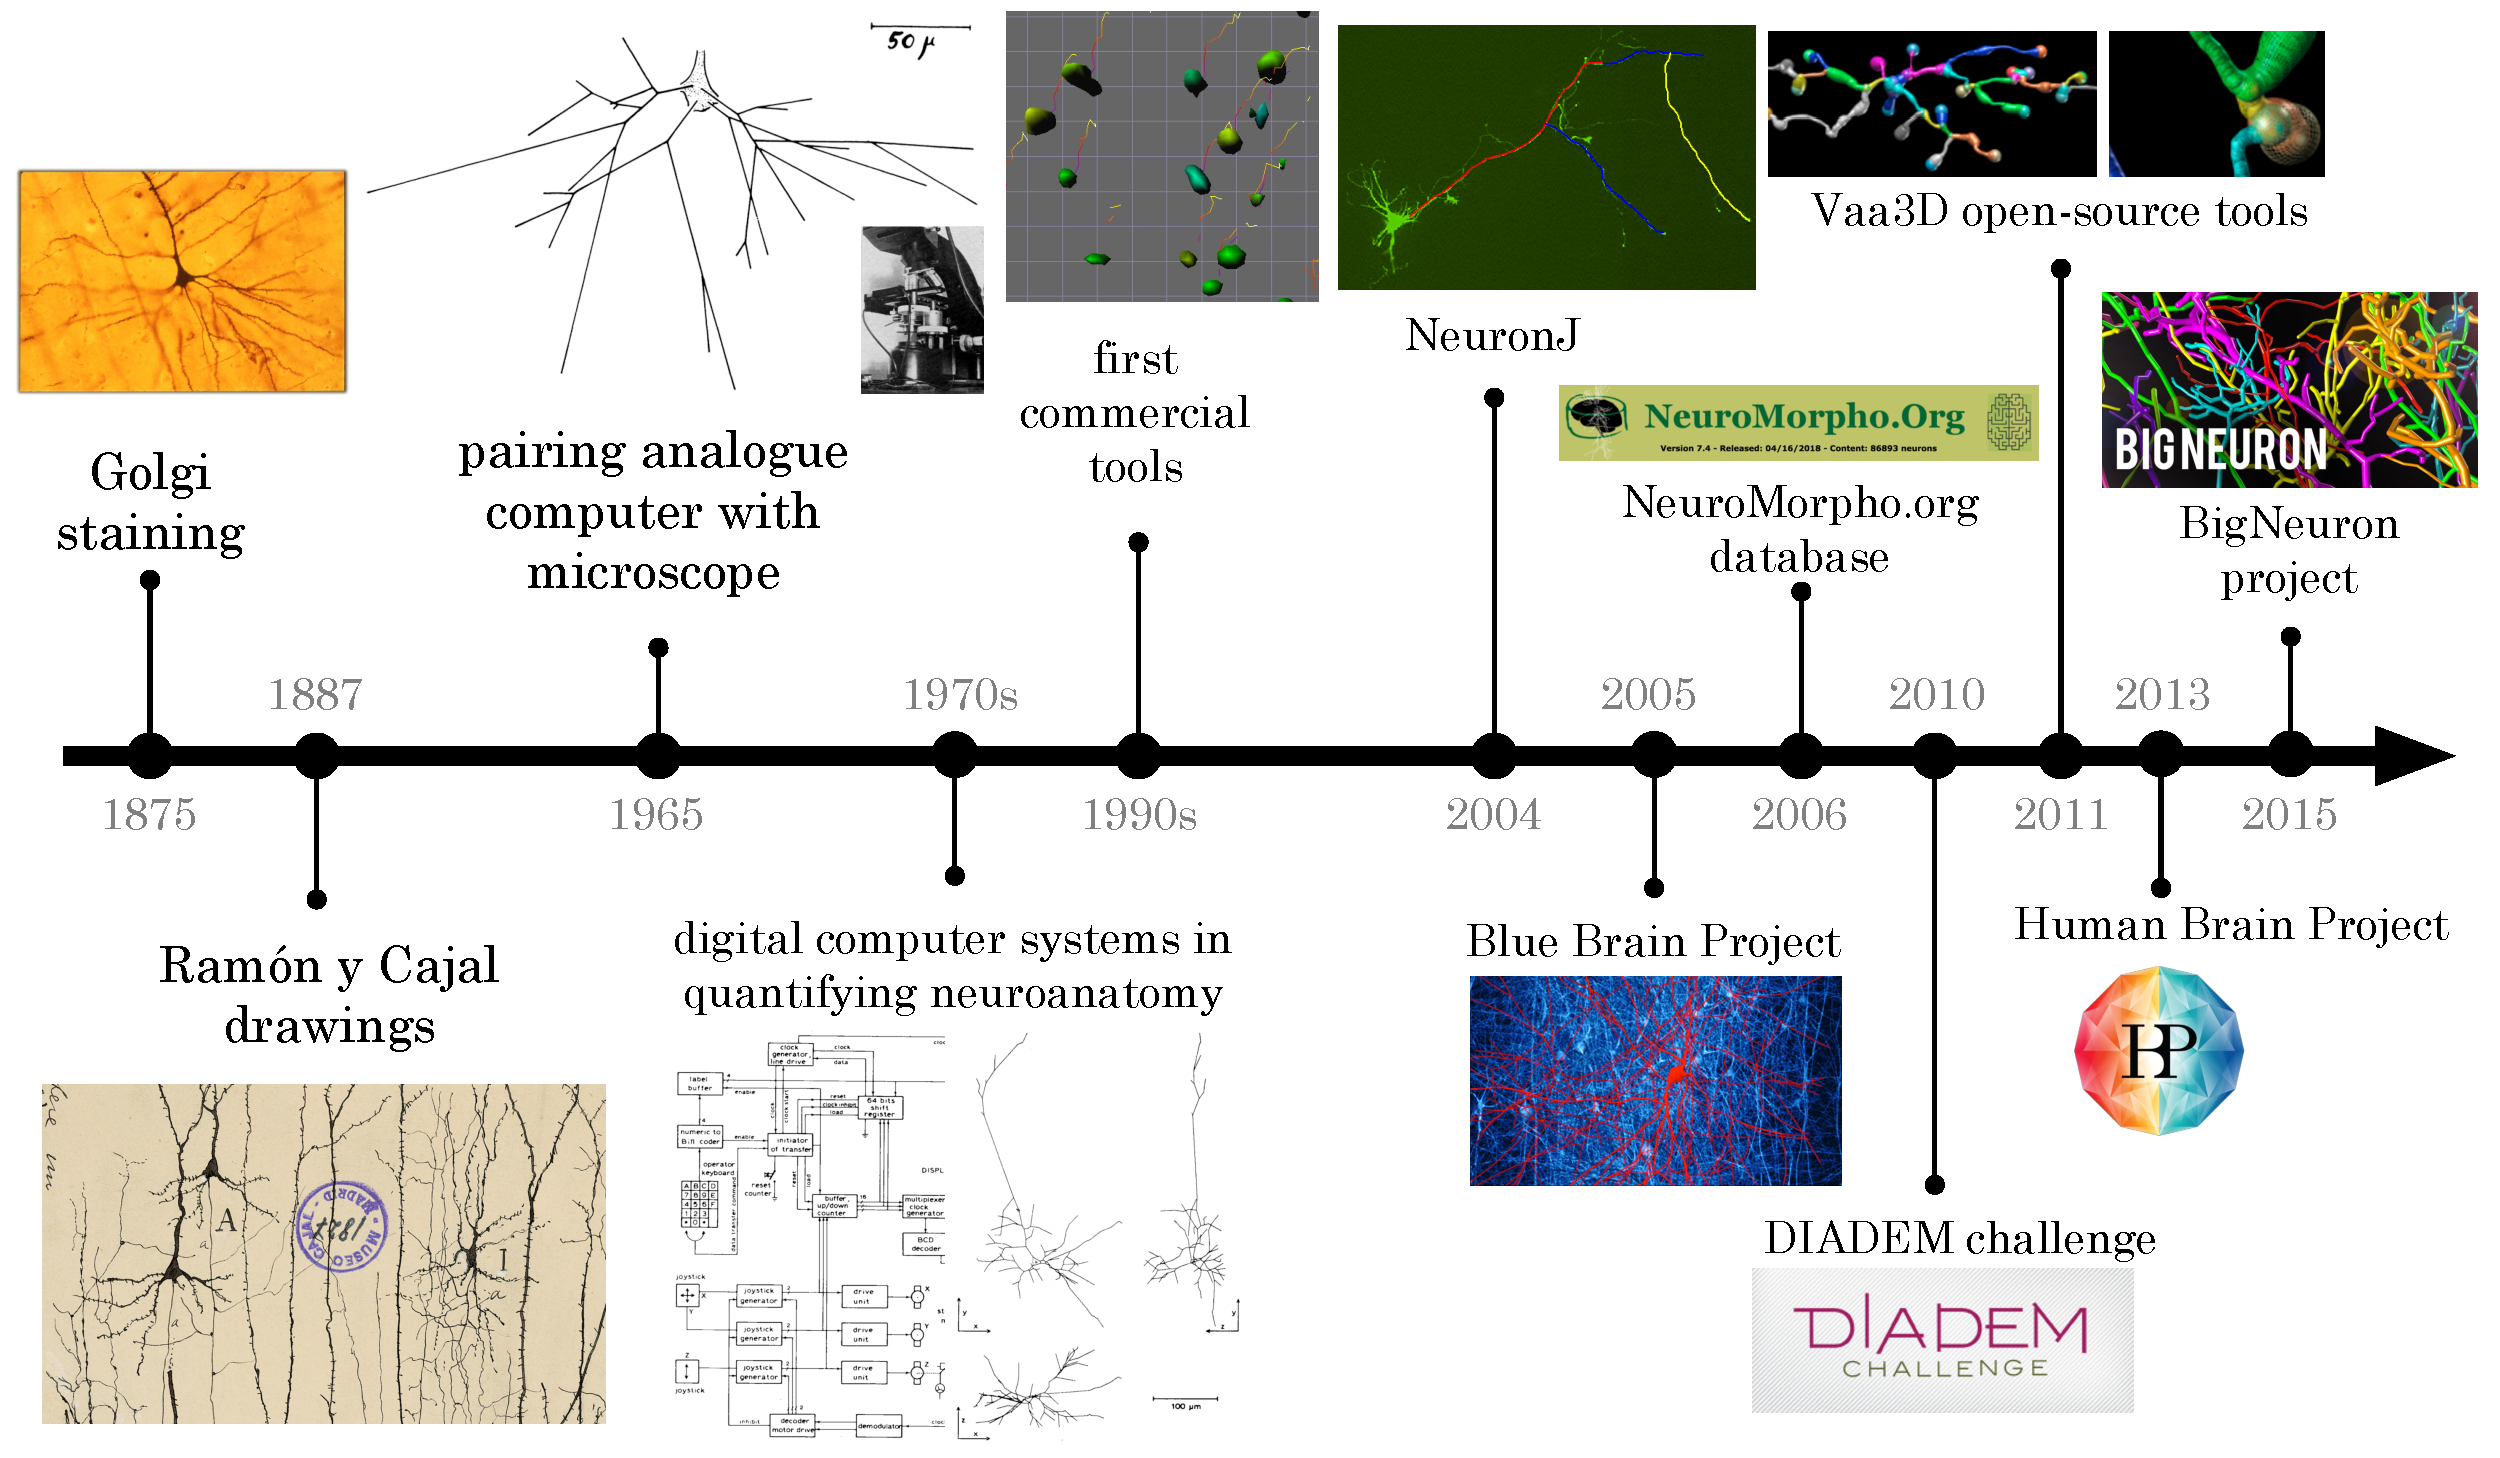
\includegraphics[width=\textwidth]{ch1_fig1}
	\end{center}
	\caption{Timeline overview of the selected relevant achievements concerning to the neuron cell analysis. The impact of the electrical engineering and the computer science is crucial for the great achievements in recent past.}
	\label{ch1_fig1}
\end{figure}

Neuron cell thus represents a core building block of the brain and the nervous system. It appears in variety of shapes (Figure~\ref{ch1_fig7}) and specializations \cite{ascolitrees}. The estimated number of neuron cells in a human brain amounts to striking 89 billion \cite{herculano2009human} - number comparable to the count of stars in the Milky Way galaxy. The dimension of each neuron can range from a few to several tens of micrometer with the neurite branch diameter typically measured in $\mu m$ scale. Each neuron is further connected to 50 thousand other neurons on average which results in an extremely powerful computational network and an very efficient information storage device. Intriguing mechanism of the brain functioning has recently emerged as an important research topic as the complex functionality of the brain defines much of the living organism activities, even the those abstract and subjective such as consciousness. Modeling the brain functionality is one of the grand unanswered questions of our era and central to diverse fields such as physics, mathematics, biology and recently prominent - computer science \cite{markram2015reconstruction}.

Neuron analysis gear has been adopting to the advancements of technical infrastructure available for the experimentation. Numerous technical obstacles have nevertheless persisted when reaching out to record the neuronal sample. This is primarily due to the physical and physiological difficulties and the generally intangible functioning mode of the nervous system. With the early analogue computers \cite{glaser1965semi}, it became possible to connect computer with microscope and automate tracing using analogue linear motion transducers as well as significantly speed up gathering of the information about the dendritic and axonal patterns. Subsequent generations of digital computers \cite{capowski1981accurate,capowski1977computer} brought further advances in the neuron reconstruction technique by introducing the computer graphics mixed with the neuron image and the advanced operator controls such as 3D joystick. The expansion of home PC hardware and software in late decades of the 20th century increased the impact of the informatics \cite{halavi2012digital}. Breakthrough of the conventional PCs made it feasible to throughput more computation and eventually implement in practice the algorithms that, although previously discovered, could not be directly implemented and shared between the users on a needed scale. It also marks the period when the first commercial and open-source academic software solutions emerge and grow (Fig.~\ref{ch1_fig1}) which to this day proved to be a steady trend.
% In decades following the emergence of neuroscience, the instrumentation has been a limiting factor to the amount and the variety of the morphologic data that could be gathered \ref{ch1_fig1}. At the beginning of the second half of the 20th century, conventional electronic analog techniques were used to join microscope and the analogue computer to automate the neuron morphology quantification.

\begin{figure}[t!]
	\begin{center}
		\includegraphics[width=\textwidth]{ch1_fig7}
	\end{center}
	\caption{Example neuronal branching arbors selected from the NeuroMorpho.org database. Showcase the topological diversity across multiple species, brain regions, and laboratories worldwide. Renderings exported using web-based neuron morphology viewer \cite{bakker2016web}.}
	\label{ch1_fig7}
\end{figure}

The crucial engineering tasks concerning the neuron reconstruction are: 1) need for the reduction of the time interval needed to compute the digital reconstruction and 2) most accurate possible reconstruction using often challenging data. The astonishing increase in the volume of acquired microscopy imaging data \cite{meijering2016imagining} undoubtedly raised the requirements bar when it comes to the time needed to for the reconstruction as images are increasingly larger and dedicated algorithms are needed to cope with the sized image volumes \cite{peng2017automatic}. Wide variety of neurons imaged under different modalities of the light microscopy (dark-field, bright-field, confocal) are still challenging for automated processing \cite{svoboda2011past,peng2011proof} and plethora of the reconstruction methods \cite{peng2011automatic} have ever since dealt with this task, resulting in two grand challenges such as DIADEM\footnote{http://diademchallenge.org} (``digital reconstruction of axonal and dendritic morphology'') and BigNeuron\footnote{http://bigneuron.org} \cite{peng2015diadem,peng2015bigneuron,gillette2011diademchallenge} (Fig.~\ref{ch1_fig1}) intended to stimulate the community effort and improve the overall state-of-the-art. In spite of the great advancements in the field, both tasks are yet very actual.

The physical appearance of the neuron cells takes part in the nervous system activity. Morphology of the single cell, shape of the neuronal network, topology or connectivity react to the external conditions or external stimuli. With the imaging tools such as fluorescence microscopy, the physical appearance the morphology of the single cell can be captured at micro meter scale can be inspected and recorded. Indeed, the studies that require deeper analysis make use of the imaging techniques that can reach nano meter scale, such as electron microscopy. In other words, accurate quantification of the cell shape is an important step towards better understanding of the cell functionality. Quantification of the neuronal structure is crucial in many neuroscience studies \cite{halavi2012digital} and quantification from microscopic images is identified as one of the major technical challenges in the digital era of neuroscience \cite{peng2015diadem}.

The advancements in informatics made it possible (Fig.~\ref{ch1_fig1}) to utilize computers to solve the neuroinformatics challenges over recent decades. With the ever growing amount of data, the processing of the information remains a challenge.   

\section{Capturing neuron morphology}
Typically, imaging neurons consists of three main stages \cite{peng2015bigneuron}. First, the neuron sample is labeled in order to expose the structure, then the digital images are acquired using one of the microscopy modalities. Finally, the obtained neuron images are computer processed. The key obstacles in reaching the accurate and robust automation of the neuron reconstruction \cite{meijering2010neuron,donohue2011automated,acciai2016automated} can be seen through the number of hampering factors which concern both the intricate nature of the data and the barriers imposed by the imaging modality. In this regard, it is possible to identify some major hurdling items.

\textit{Morphology} of the neuron cell is remarkably diverse (Fig.~\ref{ch1_fig7}). The structural intricacy of the complex examples can be challenging, even to the human visual comprehension. High complexity requires large amount of hours needed for manual delineation which thus inevitably becomes more error-prone. Hence the need for constant improvement of the computer vision algorithms. The aim of the methods is to reduce the manual labor time while fabricating trustful reconstructions. For instance, the 20-fold speedup of the reconstruction time compared to the manual reconstruction had been projected in earlier challenges \cite{liu2011diadem}.

\textit{Imaging} neurite arbor using different variations of light microscopy has been widely accepted choice for inspecting the cell structure \cite{meijering2010neuron,donohue2011automated}. Capturing $\mu$m scale objects (e.g. neurite diameter \cite{ascolitrees}), however, introduces imaging limitations. Optical systems suffer from the diffraction limit resulting in the single-lens imaged object point source being transmitted as the airy pattern \cite{cox2012optical}. In practice, the point source produces the point-spread function (PSF) which under reasonable assumptions can be approximated with the Gaussian \cite{zhang2007gaussian}. Nevertheless, the lateral resolution in fluorescence microscopy is such that the neurite dimensions are not substantially higher than the imaging resolution limits (sub-$\mu$m) which can be a limiting factor. Axial spatial resolution ($xy$ plane), on the other hand, is yet even (multiple times) lower as the precision is lost in the transition when imaging different stack layers ($z$ axis resolution). Eventually, the imaging process is predominantly affected by the particle-count driven photon noise \cite{van1998digital}, modeled with the Poisson process. Thus, the Poisson distribution is further used in generating synthetic microscopic images \cite{smal2010quantitative}. In accordance with the earlier studies, signal-to-noise ratio (SNR) of the microscopic image is expressed as the ratio of the intensity inside neuron above the background and the standard deviation of the noise inside neuron \cite{cheezum2001quantitative,smal2010quantitative}. Besides optical ``blurring'', neuron imaging can comprise pixelisation with the large spatial extent of the neuron. Combining together the optical magnification with the limited size of the digital matrix used to store the recording, as a consequence -the voxel size becomes larger that the PSF resulting in partial volume effect .
% particles and debris can be erroneously detected as neuron structures

Burden of the ever increasing \textit{data volume size} - the dimensions of the neuronal image stacks \cite{peng2017automatic} represent a hurdle for the processing and often require dedicated methods, such as processing of the stitched imagery \cite{zhou2015neuron}. The objective to stay accurate and processed in reasonable time.

\textit{Need for customization} The algorithms often need to be tailored in order to address a particular biological question and be used in wider range of the biological questions being studied which prevents them from being used across different laboratories.

\textit{Gold standard} reconstruction can differ between different experts and is not guaranteed. Attempts to reach a consensus by bringing together gold standards from different sources \cite{peng2015bigneuron}. Hence, the corrections (proof-editing) is often needed \cite{peng2011proof}. One way to overcome this is to use the consensus from the available gold-standard reconstructions, or to do the reverse engineering by generating synthetic neurons \cite{Koene-2009,radojevic2015fuzzy}
%\textit{Dynamic images} Analysis of the images captured from the live neuronal cultures.

Aforementioned factors impose much of the computational barrier \cite{svoboda2011past} in attempt to consistently produce digital reconstructions comparable with the expert ones. To have the optimal results in practice, additional expert corrections are frequently essential \cite{peng2011proof}. 

\section{Neuron tracing in light microscopy images}
Strategies in neuron tracing...
What is typically computed in neuron tracing? Centroid $\mathrm{p}(\mathrm{x} | \mathrm{y})$ Tracing is boiled down to the optimization problem, finding and optimal path (Fig.~\ref{ch1_fig2}a) or a tree (Fig.~\ref{ch1_fig2}b).


Tracing approaches (geodesic, live-wire) often (typically) involve cost function that either represents .

Live-wire, based on the established Dijkstra shortest path algorithm \cite{dijkstra1959note}.
\begin{equation}
C(\mathrm{p}_1, \mathrm{p}_2) = \gamma C_{\lambda}(\mathrm{p}_2) + (1 - \gamma) C_{\mathrm{v}}(\mathrm{p}_1, \mathrm{p}_2)
\label{ch1_eq2}
\end{equation}

\begin{equation}
C_{\lambda}({\mathrm{p}}) = \rho(\mathrm{p})
\end{equation}

\begin{equation}
C_{\mathrm{v}}(\mathrm{p}_1, \mathrm{p}_2) = \frac{1}{2} \left(  \varphi(\mathrm{p}_1, \mathrm{p}_2) + \varphi(\mathrm{p}_2, \mathrm{p}_1) \right)  
\end{equation}

\begin{figure}
	\centering
	\begin{tabular}{c@{\hspace{1em}}c@{\hspace{1em}}c@{\hspace{0.75em}}}
		\includegraphics[width=0.25\textwidth]{ch1_fig2a} & 
		\includegraphics[width=0.25\textwidth]{ch1_fig2b} & 
		\includegraphics[width=0.25\textwidth]{ch1_fig2c} \\
		a) Shortest path tracing & b) Minimum spanning tree & c) Path-pruning
	\end{tabular}
	\caption{Examples of key neuron reconstruction strategies: a) Finding optimal path having two control points, b) Inferring the  optimal tree structure from the set of nodes c) Pruning the over-complete neuron tree.}
	\label{ch1_fig2}
\end{figure}

\subsection{Bayesian methods in neuron tracing} 
Bayesian reasoning relies on the assumption that the estimated unknown quantities are hidden, not measurable directly but possible to estimate (filter) their posterior distribution using given observations \cite{doucet2001introduction}. Bayesian model consists of two essential components: prediction and update \cite{ristic2004beyond}. Prediction uses exiting prior knowledge to generate the prior distribution  of the state variable, denoted with $ \{ \mathrm{x}_t $, $ t \in \mathbb{N} \} $.  $ \{ \mathrm{y}_t, t \in \mathbb{N} \} \{ \mathrm{p}(\mathrm{x} | \mathrm{y}) \} $ 


offers a common generic solution for tasks that involve non-Gaussianity, high dimensionality, non-linear state-space model, where state-space cannot be Gaussian. Other names for the same concept are: (optimal nonlinear, stochastic). In essence, the approach boils down to computing posterior distributions of the values intended to be filtered. Basic algorithm applicable in different contexts. The problem is defined as the estimate the set of hidden states The approach is also convenient becuase it leaves plenty of possibilities for customization of the filtering (it can be used as a component algorithm).

Other methods used to establish optimal connections between paths.
The collection of the methods used: shortest path (i.e. Dijkstra \cite{dijkstra1959note}), fast marching, geodesic . In all of those an optimal solution to the cost is sought after. Currently, BigNeuron challenge Several notable approaches in broad sense can be differentiated.

On model-based reasoning. Why is the Gaussian cross-section model \cite{zhao2011automated,radojevic2017neuron} suitable.

\subsubsection{Likelihood}
Zero-mean normalized cross-correlation (ZNCC) is defined as 

\begin{equation}
c_{\mathrm{p}, \sigma} = \frac{ \sum\limits_{d\mathrm{p}} (I(\mathrm{p} + d\mathrm{p}) - \bar{I}(\mathrm{p}))(G_{\sigma}(\mathrm{p}) - \bar{G}_{\sigma}) }{ \sqrt{ \sum\limits_{d\mathrm{p}}(I(\mathrm{p} + d\mathrm{p}) - \bar{I}(\mathrm{p}))^2 \sum\limits_{d\mathrm{p}}(G_{\sigma}(\mathrm{p}) - \bar{G}_{\sigma})^2 } }
\label{ch1_eq1}
\end{equation}

\section{Tools}
One of the key Java tools is the ImageJ library \cite{abramoff2004image} with method \cite{longair2011simple,pool2008neuritetracer}. Variety of other software platforms \cite{meijering2010neuron,acciai2016automated}. 

% https://www.neuron.yale.edu/phpBB/viewtopic.php?t=3477
% http://www.neuromorpho.org/myfaq.jsp (What is SWC format?)
% http://research.mssm.edu/cnic/swc.html
% http://www.neuronland.org/NLMorphologyConverter/MorphologyFormats/SWC/Spec.html
\section{Neuronal reconstruction format}
Once processed, neurons are typically exported into a dedicated data format intended to store the idiosyncratic tree-like topology of the cell. Among different ideas and implementations of standards used for storing reconstructed neurons, two neuron morphology file formats prevail in lab usage and recent large scale neuron related projects \cite{bakker2016web}: Neurolucida DAT format (MicroBrightField, Inc.) and SWC format \cite{cannon1998line}. Neurolucida DAT format is closed-source binary format whose reverse engineered description\footnote{http://neuronland.org} suggests neuron compartments being saved as a hierarchical tree of the linear segments. SWC format on the other hand is open-source, space delimited text format that stores tree structure in an array $\mathcal{N} = \{ n_1, \dots , n_i, \dots , n_j, \dots  \}$ where each element of the array, $n_i$, corresponds to a neuronal spherical compartment (Fig.~\ref{ch1_fig5}d). SWC, therefore, renders the reconstruction as a list of nodes (neuronal compartments) with seven attributes: node index identifier $i$, node type, sphere 3D coordinates $(x_i,y_i,z_i)$, radius $r_i$ and a parent node index (Fig~\ref{ch1_fig5}). Parent node index represents the link towards predecessor node. By convention it is set to -1 for the origin node. To conform with a tree structure, each spherical compartment may have one predecessor (parent) with lower node index ($i<j$, Fig.~\ref{ch1_fig5}). Loops and disconnected branches should not exist as that would not be in agreement with the tree-like structure. Etymologically, SWC represents the acronym containing the initials of the last names of Stockley, Wheal, and Cole. Although not directly described in their joint work on quantitative measurement and modeling of the neuron morphology \cite{stockley1993system}, the origin of the SWC name is an acronym of the initials of their last names. 

Lastly, the SWC format exhibits variations, especially concerning the unified definition of the soma reconstruction \cite{bakker2016web}. Several interpretation of the standard exist\footnote{http://research.mssm.edu/cnic/swc.html}\footnote{http://www.neuronland.org/NLMorphologyConverter/MorphologyFormats/SWC/Spec.html}\footnote{NeuroMorpho.org FAQ: What is SWC format? http://www.neuromorpho.org/myfaq.jsp}. One of the downsides of the SWC format is its often oversimplified cylinder model of the soma. Being a rather simple (straightforward to implement the software to read and export) and open-source format, easy for exchange - it has been adopted by notable large-scale neuron morphology projects \cite{ascoli2007neuromorpho,peng2015bigneuron}.

The work showcased in this thesis will exclusively use open source SWC format.
 
\begin{figure}
\begin{center}
	\begin{tabular}{c@{\hspace{0.75em}}c@{\hspace{0.75em}}c@{\hspace{0.75em}}c@{\hspace{0.75em}}}
	\includegraphics[align=c,width=0.2\textwidth]{ch1_fig5a} & 
	\includegraphics[align=c,width=0.2\textwidth]{ch1_fig5b} & 
	\includegraphics[align=c,width=0.2\textwidth]{ch1_fig5c} &
	\includegraphics[align=c,width=0.2\textwidth]{ch1_fig5d} \\ 
	a) & b) & c) & d)
\end{tabular}
\end{center}
	\caption{Neuron morphology digital format data structure: a) Single neuron image, b) Digital reconstruction of the given neuron c) Illustration of the SWC format \cite{cannon1998line} used to store the digital reconstruction idiosyncratic tree structure $\mathcal{N} = \{ n_1, ... , n_i,..., n_j, ... \}$, d) Detailed visualization of the linear segment (truncated cone) connected pair of neuron compartments $(n_j, n_i)$ along with the component elements. Reconstruction exported using web-based neuron morphology viewer \cite{bakker2016web}.}
	\label{ch1_fig5}
\end{figure}

Measuring distances between neurons: L-measure \cite{scorcioni2008measure}, Neuro-blast \cite{wan2015blastneuron}. Distances between neurons can be based on the overlap and the inter-node metric distances.

\section{Thesis outline}

\subsubsection{Fuzzy logic system}
Detecting characteristic points of the neuron tree structure, along with many of the concepts encountered in various domains of human knowledge, is in practice, too complex to be modeled with a concise or precise definition. This is true, for example, for expressing . Unsupervised method based on fuzzy logic, linguistic variables and set of if-then rules is used to 

dealing with such concepts through the use of fuzzy algorithms structured as a branching questionnaire.

Usage of the linguistic variables 

\subsubsection{Multiple hypothesis tracking}
Computation methods

Chapters include synthetic images that offer possibility of objective comparison.

This thesis primarily addresses/contributes to the need for automated methods for neuron reconstruction. 
In this thesis, methods that cope with uncertainty are showcased. The work is showcased in the domain of the neuron reconstruction and several neuron related tasks such as the object detection, namely the detection of the critical points (bifurcation and terminal) in microscopic images of neurons (Chapter~\ref{ch2:fuzzy}) and the localization  The first chapter  and probabilistic and bayesian methods are explored. The underlying idea assumes that the neuron tracing itself is never a .

The thesis is organized as follows. In Chapter 2,  . Subsequently, in Chapter 3, 

